\documentclass[12pt]{article}
\usepackage{ctex}
\usepackage[english]{babel}
\usepackage{blindtext}
\usepackage{nameref}
\usepackage{fancyhdr}
\usepackage{amsmath,amssymb,amsthm}
\usepackage{graphicx,float}
\usepackage{physics}
\usepackage{pgfplots}
\usepackage[a4paper, total={6in, 9in}]{geometry}

\graphicspath{ {../images/} }

\pagestyle{fancy}
\fancyhf{}
\fancyhf[HL]{Quadratic equations in one unknown}
\fancyhf[CF]{\thepage}

\newcommand{\innerprod}[2]{\langle{#1},{#2}\rangle}
\newcommand{\id}{\mathtt{id}}

\newtheorem*{definition}{Definition}
\newtheorem*{theorem}{Theorem}
\newtheorem*{corollary}{Corollary}
\newtheorem*{lemma}{Lemma}
\newtheorem*{proposition}{Proposition}
\newtheorem*{remark}{Remark}
\newtheorem*{claim}{Claim}
\newtheorem*{example}{Example}
\newtheorem*{axiom}{Axiom}

\begin{document}
    \section*{Learning objectives}
    By studying this unit, we will achieve the following goals:
    \begin{enumerate}
        \item Solving quadratic equations by the factor methods.
        \item Forming quadratic equations from given roots.
        \item Solving the equation $ax^2+bx+c=0$ by plotting the graph of the parabola $y=ax^2+bx+c$ and reading the x-intercepts.
        \item Solving quadratic equations by the quadratic formula.
        \item Understanding the relations between the discriminant of a quadratic equation and the nature of its roots.
        \item Solving problems involving quadratic equations.
        \item Understanding the relations between roots and coefficients and form quadratic equations using those relations.
        \item Appreciating the development of the number systems including the system of complex numbers.
        \item Performing addition, subtraction, multiplication and division of complex numbers.
    \end{enumerate}
    \section*{Background}
    It was a long time ago that we may not determine when did humanity started to examine quadratic equation, but it was already known to ancient Egyptians. Here, we recall some basic algebraic operations and think of a question.

    We recall the algebraic expressions we learned in junior secondary, and read the following problem.
    
    `Given a rectangle of perimeter $p$ and area $a$, how long should its side lengths be?'

    In order to solve the above problem, we may need to let $x$ and $y$ to be its side lengths. Converting the words into algebraic expressions gives us the following system of simultaneous equations:
    \begin{align*}
        \begin{cases}
            x+y=p\\xy=a
        \end{cases}
    \end{align*}
    
    To be simpler, we may fix some number for $p$ and $a$, so that the problem looks easier to solve - we could literally focus on the unknowns, where we may adopt the similar deduction from the simplified case to general case.

    Let's pick $p=1$ and $a=1$ for instance, which looks simpler. And now the system becomes
    \begin{align*}
        \begin{cases}
            x+y=1\\xy=1
        \end{cases}
    \end{align*}

    The genius from history thought of the solution using substitution, through transforming the system of two unknown into one first, then solve for the other using the deduced relations. Now, we may take a look at the second equation in the system, which can be modified as $$xy=1\implies y=\frac{1}{x}$$ as long as $x\neq0$ and $y\neq0$. In fact, it must not be happening since if $x=0$ or $y=0$, $xy=0$ in which it falsified the system argument. We then substitute $y=\frac{1}{x}$ into the first equation to form the new argument in one unknown:
    \begin{align*}
        x+(\frac{1}{x})&=1&&(\textrm{sub }y=\frac{1}{x})\\
        x(x+\frac{1}{x})&=x(1)&&(\textrm{multiply both sides by }x)\\
        x^2+1&=x\\
        x^2-x+1&=0
    \end{align*}
    where it comes to the stopping point. This is where we starts the discussion of quadratic equation.

    \section*{Factor method}
    One observed that, to solve some quadratic equations (some but not all, you will figure out why later), we have the knowledge to construct the following: $$(x-\alpha)(x-\beta)=x^2-(\alpha+\beta)x+\alpha\beta$$ which, in fact, satisfy the form of a quadratic equation. We may also notice the fact that solving $(x-\alpha)(x-\beta)=0$ is much easier than seeing the original quadratic form. We then exhibit the following:
    \begin{theorem}
        If $ab=0$, then $a=0$ or $b=0$.
    \end{theorem}

    The meaning of this theorem is that, we must have either one of the factor being 0 if the product of them is zero. You may think it naturally that 0 dominant other numbers.

    Therefore, we can apply this theorem to the problem $(x-\alpha)(x-\beta)=0$, and we may deduce that 
    \begin{align*}
        x-\alpha=0&&\textrm{or}&&x-\beta=0\\
        x=\alpha&&\textrm{or}&&x=\beta
    \end{align*}

    The above result is cool, but the difficulties are still existing. We are still looking for the way to perform factorization. One suggested the usage of cross method.

    The cross method is literally a testing by exhausting every possible results and choose the suitable one as the answer. For example, we may look at $x^2-5x+6=0$. We shall see $6=1\times 6=2\times 3=-1\times -6=-2\times -3$. As we see from previous page, we need the middle term to be $-5x$, which means $\alpha+\beta=5$. The pair that satisfies this result is 2 and 3, so the factor form becomes $(x-2)(x-3)=0$, and solved by $x=2$ or $x=3$.

    But this turns out that we are in fact not seeing the quadratic equation itself but eventually returning the situation 
    \begin{align*}
        \begin{cases}
            \alpha+\beta=5\\
            \alpha\beta=6
        \end{cases}
    \end{align*}
    with the method of testing, which is not a good practice, and not a reasonable system we want. We must see the factor method is not effective enough to draw out solutions for all cases. 

    \section*{Forming quadratic equations from given roots}
    Alternatively, and for the sake of seeing why factor method is not effective enough, we may acquire the concepts of forming quadratic equations using given roots.

    Recalling the relation from above, we may see that $$(x-\alpha)(x-\beta)=x^2-(\alpha+\beta)x+\alpha\beta$$ gives us the concrete formula to construct a quadratic equation using given roots. We may simply plug the roots in $\alpha$ and $\beta$ respectively. For instance, if we choose to pick complicated numbers as roots, we will see why not every quadratic equation could be solved using cross method, as we are not able to directly guess such monsters. Let's check the following:
    \begin{enumerate}
        \item $\alpha=\frac{2}{7}, \beta=\frac{7}{2}\implies 14x^2-53x+14=0$
        \item $\alpha=1+\sqrt{2}, \beta=1-\sqrt{2}\implies x^2-2x-1=0$
    \end{enumerate}
    
    We have no capability of these kinds of monster numbers, at least we could not directly get to the solutions. It proves the limitation of factor method.

    \section*{Graphical solution to quadratic equation}
    One suggested the thought of graphing, in which we should have learned the technique of plotting a graph in junior secondary. Let's recall the memory of it first.

    Consider we have a coordinate plane, and our coordinate are presented in the form of an ordered pair $(x,y)$. We set the relation $y=ax^2+bx+c$, for instance, $y=x^2-2x-1$. Observe some of the values of this equation, and we may use a table to write them down:
    \begin{center}
        \begin{tabular}{|c||c|c|c|c|c|}
            \hline
            x&-2&-1&0&1&2\\
            \hline
            y&7&2&-1&-2&-1\\
            \hline
        \end{tabular}
    \end{center}

    We could observe that $y=2>0$ when $x=-1$, and $y=-1<0$ when $x=0$. So there must be some $x$ between $-1$ and $0$ so that $y=0$, ensured by a solid theorem called Mean Value Theorem. It turns out the solution to the quadratic equation exists. Why is this so? As we consider $y=ax^2+bx+c$, we are observing a more general case of the problem. In particular, the scenario for $y=0$ returns to the quadratic equation, and our work before provided information for the existence of $y=0$, so there is some $x$ satisfying the condition, which indeed is concluding the existence of solution.

    May we complete the graphical method in following way. We first plot the points calculated before. They are $(-2,7),(-1,2),(0,-1),(1,-2),(2,-1)$ according to the table. We then have the following graph:\\
    \begin{center}
        \begin{tikzpicture}
            \begin{axis}[
            axis lines = left,
            xlabel = \(x\),
            ylabel = {\(y\)},
            xmin=-3, xmax=3,
            ymin=-3, ymax=8,
            xtick={-3,-2,-1,0,1,2,3},
            ]
            \addplot+ [nodes near coords,only marks,
            point meta=explicit symbolic]
            table [meta=label] {
            x y label
            -2 7 (-2,7)
            -1 2 (-1,2)
            0 -1 (0,-1)
            1 -2 (1,-2)
            2 -1 (2,-1)
            };
            \end{axis}
        \end{tikzpicture}            
    \end{center}

    We shall link the points up, and with some smoothness, we may draw the graph like:
    \begin{center}
        \begin{tikzpicture}
            \begin{axis}[
            axis lines = left,
            xlabel = \(x\),
            ylabel = {\(y\)},
            xmin=-3, xmax=3,
            ymin=-3, ymax=8,
            xtick={-3,-2,-1,0,1,2,3},
            ]
            \addplot+ [nodes near coords,only marks,
            point meta=explicit symbolic]
            table [meta=label] {
            x y label
            -2 7 (-2,7)
            -1 2 (-1,2)
            0 -1 (0,-1)
            1 -2 (1,-2)
            2 -1 (2,-1)
            };
            \addplot [
                domain=-3:3, 
                samples=100, 
                color=red,
            ]
            {x^2 - 2*x - 1};
            \end{axis}
        \end{tikzpicture}            
    \end{center}

    And we observe that solving $x^2-2x-1=0$ is equivalent to solve the system
    \begin{align*}
        \begin{cases}
            y=x^2-2x-1\\
            y=0
        \end{cases}    
    \end{align*}
    which, we can put the line $y=0$ on the graph to search for the intersections, as we knew the solution to the system of equations are the intersections of the equations. Hence, we have\\
    \begin{center}
        \begin{tikzpicture}
            \begin{axis}[
            axis lines = left,
            xlabel = \(x\),
            ylabel = {\(y\)},
            xmin=-3, xmax=3,
            ymin=-3, ymax=8,
            xtick={-3,-2,-1,0,1,2,3},
            ]
            \addplot [
                domain=-3:3, 
                samples=100, 
                color=blue,
            ]
            {x^2 - 2*x - 1};
            \addlegendentry{$y=x^2-2x-1$}
            \addplot[
                domain=-3:3,
                samples=100,
                color=red
            ]{0};
            \addlegendentry{$y=0$}
            \end{axis}
        \end{tikzpicture}            
    \end{center}

    Here, we can observe the intersections lie in between $-1$ to $0$ and $2$ to $3$. They are the desired roots, a.k.a. solutions, to the quadratic equation. This is the visualisation to quadratic equation in some sense. But one could still not easily determine the roots of the quadratic equation explicitly from the graph. We still need other effective thinking to achieve the goal.

    \section*{The quadratic formula}
    Modern society equipped with modern tools. The explicit solution usually exists in algebraic ways, because algebraic expressions are meaningful in expressing thoughts. We could now study two of the genius thinking to solve \textbf{any} quadratic equation effectively.

    \subsection*{Completing square}
    One should see if $x^2=c$ with $c\geq0$ constant, then $x=\pm\sqrt{c}$. We adopt the meaning of $\pm$ as `plus or minus'. The historical genius thought that if they could complete a square from the original equation, then they would be able to resolve the problems. Recall the identity $$(a+b)^2\equiv a^2+2ab+b^2$$ such that we are able to see $x=a$ and remain to find what $b$ substitutes. Let's check a simpler case (monic case) of a quadratic equation: $$x^2+px+q=0$$

    We shall compare the like terms and retrieve the condition $p=2b$ such that there is a complete square to simplify the variables. We have the following trick:
    \begin{align*}
        0=x^2+px+q&=x^2+2(\frac{p}{2})x+q\\
        &=x^2+2(\frac{p}{2})x+(\frac{p}{2})^2-(\frac{p}{2})^2+q\\
        &=(x+\frac{p}{2})^2+q-\frac{p^2}{4}
    \end{align*}
    Then,
    \begin{align*}
        (x+\frac{p}{2})^2&=\frac{p^2}{4}-q\\
        (x+\frac{p}{2})^2&=\frac{p^2-4q}{4}\\
        x+\frac{p}{2}&=\pm\sqrt{\frac{p^2-4q}{4}}\\
        x&=\frac{-p\pm\sqrt{p^2-4q}}{2}
    \end{align*}

    We can next consider the more general case of quadratic equation $$ax^2+bx+c=0$$ with $a\neq 0$ and $b,c$ be constants. With the previous work, the simplification is simple:
    \begin{align*}
        ax^2+bx+c&=0\\
        x^2+\frac{b}{a}x+\frac{c}{a}&=0\\
        \implies x&=\frac{-b/a\pm\sqrt{(b/a)^2-4(c/a)}}{2}\\
        &=\frac{-b\pm\sqrt{b^2-4ac}}{2a}
    \end{align*}

    Hence, the solutions could be deduced using coeficients of the quadratic equation. This is called the quadratic formula. The formula is useful and we will emphasis the content later.

    \subsection*{Lagrange resolvent}
    Another method to find the quadratic equation is by the Lagrange resolvent, which is quite abstract but powerful. We recall the relation $$(a+b)^2-(a-b)^2=4ab\implies(a-b)^2=(a+b)^2-4ab$$
    
    Also, from the part of forming equations, we knew that if $$x^2+px+q=(x-\alpha)(x-\beta)$$ then $$p=-(\alpha+\beta), q=\alpha\beta$$ by comparing like terms. More about coefficients and roots will be emphasis in later sections.

    We may consider the following:
    \begin{align*}
        \begin{cases}
            r_1=\alpha+\beta\\
            r_2=\alpha-\beta
        \end{cases}
    \end{align*}
    in which we can easily see $\alpha=\frac{r_1+r_2}{2}$ and $\beta=\frac{r_1-r_2}{2}$. It suffices to resolve $r_1$ and $r_2$. 

    It is easy to see $r_1=-p$, and for $r_2$, we use the identity $r_2^2=(\alpha-\beta)^2=(\alpha+\beta)^2-4\alpha\beta=p^2-4q$. Hence, $r_2=\pm\sqrt{p^2-4q}$.

    Finally, we conclude $\frac{-p\pm\sqrt{p^2-4q}}{2}$ the quadratic formula of monic case. The general case is similar to previous method.

    \section*{Discriminant}
    Throughout the process, we have the quadratic formula $$\frac{-b\pm\sqrt{b^2-4ac}}{2a}$$ as the solution to the quadratic equation $ax^2+bx+c=0$. Observe the formula has a square root operation, which is not defining for negative numbers.

    It is interesting that if we apply the above thinking to the quadratic formula, we will have 3 cases: (1) if $b^2-4ac>0$, then there are two distinct roots; (2) if $b^2-4ac=0$, there will be double roots, or we call it only one root; (3) if $b^2-4ac<0$, the square root broke, and no solution can be found. In fact, we focus on real solution and results follow.

    We extensively define $\Delta=b^2-4ac$ for quadratic equation usage, and this will be convenient to deal with when there is more than one quadratic function to be considered.

    As a consequence, we could now write the components separately as: for $ax^2+bx+c=0$, we have $$x=\frac{-b\pm\sqrt{\Delta}}{2a}$$ where $\Delta=b^2-4ac$ is the discriminant of the quadratic equation.

    \section*{Extending to complex numbers}
    Notice that our discussion has been focused on real numbers, that we assumed that negative numbers could not be square-rooted. One observed that we are missing the completeness of rooting operations, that if we could find something that could be squaring to negative numbers, it will be perfect to talk about the general number of roots for quadratic equations, as well as higher degree polynomials.

    As we know the roots of a quadratic equation can be presented using quadratic formula, and the halting point of the quadratic formula is when the discriminant becomes negative. How should we deal with it? One suggested that we could `create' a new symbol so that we can solve for negative square roots, i.e. $x^2=-1$, where we usually observe for the case of 1. The symbol is called an \textbf{imaginary number} $i$, such that $i^2=-1$.

    Many of the public remember the symbol $i$ as $i=\sqrt{-1}$, in which many school textbooks wrote that down as the definition. However, it is wrong. We want a solution for the equation $x^2=-1$, but we don't know whether the solution is positive or negative, and in fact, we could not write about the sign of such solution as $i$ has no direction on the real line. That's why we would like to call it imaginary, because the number $i$ itself does not contain any information on positivity.

    As long as we define $i$ to be the solution of $x^2=-1$, we may notice that $-i$ also satisfies the equation $x^2=-1$, as we know $(-1)^2=1$. The meaning of the negative sign here will no longer be the direction as if in real line, but we will extend its meaning by the implication of `opposite side'. We could use an argand diagram to draw it out.

    \begin{figure}[H]
        \centering
        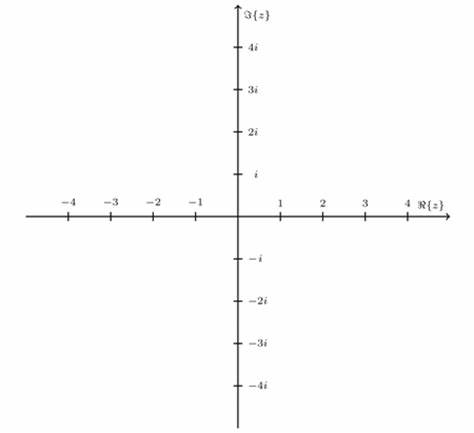
\includegraphics[scale=0.8]{argand.jpg}
    \end{figure}

    The horizontal axis denotes the usual real line, and the vertical axis denotes the imaginary line, where the two axis spans the whole argand diagram, which we call it the \textbf{complex plane}. We may here observe that $i$ does not lie on the real line, and thus we may not be able to talk about $i=\sqrt{-1}$ because we are really unable to determine its positivity. But we could still denote the opposite direction of $i$ as $-i$, which gives a broader meaning to mathematical symbols.

    For instance, we know that $i^2=-1$, so that when we are facing $x^2=-c$, where $c$ is a constant, we could write $x=i\sqrt{c}$ or $x=-i\sqrt{c}$ as our solution. This gives further information about number of roots to quadratic equation. We shall claim that any quadratic equation has at most 2 distinct roots, including complex roots. In higher mathematics, we will say it must have 2 roots, counted with multiplicity.

    \section*{The development of the number systems}
    One should feel that our number systems are developed well according to wide usages, and the development is called completion if we see the action of extending number systems as completing the tools for solving equations.

    In fact, we start from natural numbers. We could only perform addition and multiplication in it. We then have negative numbers and the zero, which makes the number system being `complete' under subtraction. We then complete the number system for division, using the fractional representation, and is called the rational number system. From Pythagoras theorem, we know that there are some numbers that could not be represented using fractional form, so we call those numbers the irrational numbers. Combining rationals and irrationals gives us the usual number system, the real number system, with literally every constructible number using compass and ruler. In higher mathematics, we know that real number system is the largest number system preserves ordering. Then we develop the completion of real numbers, which is the complex number system, through the research of solving quadratic equations.

    \section*{Arithmetic operations on complex numbers}
    For arithmetic, we simply take $i$ as algebraic variables, and remember not to do magic with real numbers. There is a separation between real and imaginary part. That is, we can write complex numbers as $$z=x+yi$$ where $z$ is the complex numebr itself, $x,y$ ar real numebrs and $x=\Re{z}$, $y=\Im{z}$. And the above presentation format is called the standard form.
    
    The arithmetic operations goes like:
    \begin{itemize}
        \item Addition: $(a+bi)+(c+di)=(a+c)+(b+d)i$, which is simply adding numbers part by part.
        \item Subtraction: $(a+bi)-(c+di)=(a-c)+(b-d)i$, similar to how addition does.
        \item Multiplication: $(a+bi)(c+di)=ac+bci+adi+bdi^2=(ac-bd)+(bc+ad)i$.
        \item Division: $\frac{a+bi}{c+di}=\frac{a+bi}{c+di}\cdot \frac{c-di}{c-di}=\frac{(a+bi)(c-di)}{c^2-d^2i^2}=\frac{ac+bd}{c^2+d^2}+\frac{bc-ad}{c^2+d^2}i$, where it rationalized the fraction to return to standard form.
    \end{itemize}
    
    We also have some more operations to categorize complex numbers from real numbers:
    \begin{itemize}
        \item Complex conjugate: $\overline{z}=x-yi$. It is like to multiply $-1$ to the imaginary part.
        \item Modulus: $|z|=\sqrt{x^2+y^2}$. It is, in some sense, the distance (length) function of a complex number.
    \end{itemize}

    \section*{Chapter exercise}
    \subsection*{Level 1}
    \begin{enumerate}
        \item Solve the following quadratic equations using factor method, graphing method and quadratic formula respectively.\begin{enumerate}
            \item $x^2-2x+1=0$
            \item $x^2-6x+9=0$
            \item $x^2-5x+6=0$
            \item $x^2-6x+5=0$
            \item $x^2-8x+12=0$
            \item $x^2+4x-32=0$
            \item $x^2-5x-84=0$
            \item $2x^2-5x+2=0$
            \item $5x^2-50x+125=0$
            \item $7x^2+75x-22=0$
        \end{enumerate}
        \item Construct 3 quadratic equations that has distinct real roots, double root, and no real roots respectively. Prove the propositions using discriminant.
        \item Solve the rectangle problem stated at the beginning of the notes.
    \end{enumerate}

    \subsection*{Level 2}
    \begin{enumerate}
        \item Show that if we have $ax^2+bx+c=0$ with $a\neq 0$ and $c\neq 0$, then $x\neq 0$.
        \item Show that if $x_1$ and $x_2$ are roots of $ax^2+bx+c=0$, then $\frac{1}{x_1}$ and $\frac{1}{x_2}$ are roots of $cx^2+bx+a=0$.
        \item Given $x_1$ and $x_2$ are roots of $ax^2+bx+c=0$, find the quadratic equation having roots $x_1^2$ and $x_2^2$.
        \item Expand $(x+a)^3$. Discuss how to make a first step to solve cubic equation $x^3+px^2+qx+r=0$.
        \item Given $\Delta_1$ and $\Delta_2$ the discriminants of $x^2+p_1x+q_1=0$ and $x^2+p_2x+q_2=0$ respectively. Define $\Delta_0$ be the discriminant of $x^2+(p_1+p_2)x+(q_1+q_2)=0$. Find an equation to relate $\Delta_0,\Delta_1,\Delta_2$. Discuss the condition for $\Delta_0=\Delta_1+\Delta_2$, and solve $x^2+p_1x+q_1=0$ and $x^2+p_2x+q_2=0$ under that condition.
        \item By completing square, find the general solution of $(a+bi)z^2+(c+di)z+(e+fi)=0$. Can we represent every solution using complex numbers? This is called algebraic closure in the field of algebra.
    \end{enumerate}

    \subsection*{Challenges}
    \begin{enumerate}
        \item Prove the theorem in Factor method.
        \item If $ax^2+bx+c=0$ has double root, at the same time $c$ is a root of the equation $x^2+4ax-bc=0$, solve for $x$ in terms of golden ratio $\varphi=\frac{1\pm\sqrt{5}}{2}$. 
    \end{enumerate}
\end{document}